\documentclass{article}
\usepackage{tikz}
\usepackage[margin=1in]{geometry} % full-width
\usepackage{graphicx}

\usepackage{listings}
\lstset{
    language=caml
}
% AMS Packages
\usepackage{amsmath}
\usepackage{amsthm}
\usepackage{amssymb}

% Unicode
\usepackage[utf8]{inputenc}


\usetikzlibrary{arrows.meta}
\newcommand {\axes}[4] {\draw[->] (0,0) -- (#3,0) node [right]{#1};
                        \draw[->] (0,0) -- (0,#4) node[above]{#2};}
\newcommand {\valx}[2] {\draw (#1,0.03) -- (#1,-0.03) node[anchor=north]{#2};}
\newcommand {\valy}[2] {\draw (0.03,#1) -- (-0.03,#1) node[anchor=east]{#2};}

\title{TIPE Sur l'optimisation du trafic routier.}
\author{MOULAT Mattéo\\NODET Gaëtan\\DURAND Ulysse\\MARGUET Emeric}
\everymath{\displaystyle}
\date{}
\begin{document}

\maketitle

Dans le monde d'aujourd'hui, le transport routier représente une grande part des
émissions de gaz à effet de serre et est aussi la cause, en france, de plus de
50 000 accidents par an. C'est pourquoi il est plus qu'important de considérer
la limitation du trafic routier.\\
Nous allons nous placer dans un monde où les véhicules suivent le chemin que
notre algorithme leur indique, et nous allons concevoir cet algorithme afin de
fluidifier le trafic routier en minimisant le temps de trajet des véhicules.


\section{Modèle} 

Le réseau routier sera un graphe orienté où les sommets sont des croisements et
les arrêtes des portions de route.
Une route à double sens est représentée par deux arrêtes distinctes.
Les voitures vont toutes d'un sommet A du graphe à un autre sommet B.
Pour une voiture, le temps de parcours d'un croisement  est nul.
Nous considérerons des débits de voiture (voitures/seconde) sur chaque portion
de route sans que ces derniers varient en fonction du temps.\\
Nous supposerons sur tout le réseau routier, la densité de voitures est la même
(voitures/m), ainsi nous pourrons modéliser les ralentissements sur une route
par une fonction appelée fonction de ralentissement de la route donnant le temps de
parcours de la route en fonction du débit entrant dans cette dernière.
L'objectif est de minimiser le temps de parcours moyen des voitures.\\
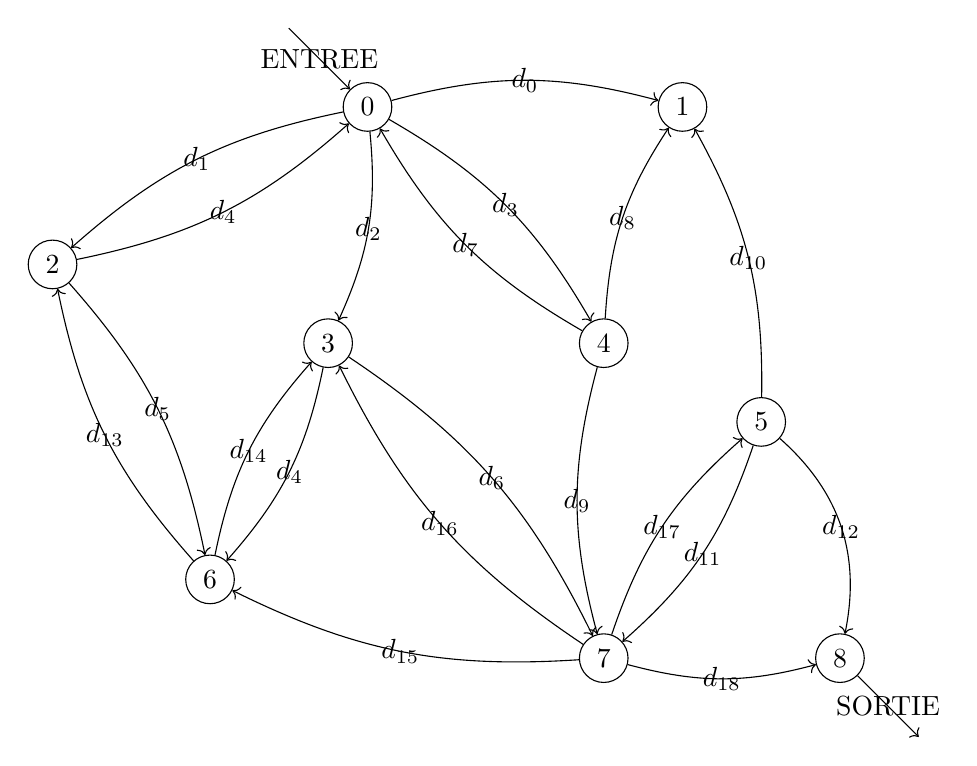
\begin{tikzpicture}
    \node[shape=circle,draw=black] (A) at (3,3) {6};
    \node[shape=circle,draw=black] (B) at (1,7) {2};
    \node[shape=circle,draw=black] (C) at (5,9) {0};%A%
    \node[shape=circle,draw=black] (D) at (4.5,6) {3};
    \node[shape=circle,draw=black] (E) at (8,2) {7};
    \node[shape=circle,draw=black] (F) at (8,6) {4};
    \node[shape=circle,draw=black] (G) at (9,9) {1};
    \node[shape=circle,draw=black] (H) at (10,5) {5};
    \node[shape=circle,draw=black] (I) at (11,2) {8};%B%
    \draw [->](4,10) -- node{ENTREE} (C);
    \draw [->](A) to[bend left=15] node {$d_{13}$} (B);
    \draw [->](B) to[bend left=15] node {$d_5$} (A);
    \draw [->](A) to[bend left=15] node {$d_{14}$} (D);
    \draw [->](D) to[bend left=15] node {$d_4$} (A);
    \draw [->](C) to[bend right=15] node {$d_1$} (B);
    \draw [->](B) to[bend right=15] node {$d_4$} (C);
    \draw [->](C) to[bend left=15] node {$d_2$} (D);
    \draw [->](C) to[bend left=15] node {$d_3$} (F);
    \draw [->](E) to[bend left=15] node {$d_{15}$} (A);
    \draw [->](F) to[bend left=15] node {$d_7$} (C);
    \draw [->](C) to[bend left=15] node {$d_0$} (G);
    \draw [->](D) to[bend left=15] node {$d_6$} (E);
    \draw [->](E) to[bend left=15] node {$d_{16}$} (D);
    \draw [->](F) to[bend right=15] node {$d_9$} (E);
    \draw [->](F) to[bend left=15] node {$d_8$} (G);
    \draw [->](E) to[bend left=15] node {$d_{17}$} (H);
    \draw [->](H) to[bend left=15] node {$d_{11}$} (E);
    \draw [->](E) to[bend right=15] node {$d_{18}$} (I);
    \draw [->](H) to[bend right=15] node {$d_{10}$} (G);
    \draw [->](H) to[bend left=30] node {$d_{12}$} (I);
    \draw [->](I) -- node{SORTIE} (12,1);
\end{tikzpicture}
\newpage
\subsection{Quelques exemples de fonctions de de ralentissement}

%%%%%%
\begin{tikzpicture}[scale=3]
    \axes{d}{t}{1}{0.6}
    \valx{0.9}{$d_{max}$}
    \valy{0.5}{$t_{max}$}
    \draw[{}-{Arc Barb [reversed]},line width = 0.3mm, color=red] (0,0.5)
             -- (0.9,0.5);
\end{tikzpicture}
%%%%%
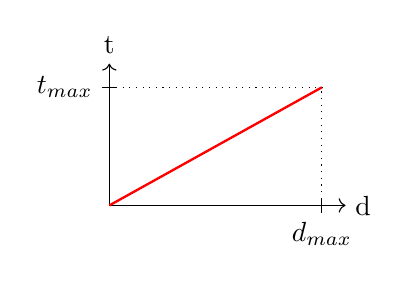
\begin{tikzpicture}[scale=3]
	\axes{d}{t}{1}{0.6};
	\valx{0.9}{$d_{max}$};
	\valy{0.5}{$t_{max}$};
	\draw[line width = 0.3mm, color=red] (0,0)--(0.9,0.5);
	\draw[dotted] (0.9,0) -- (0.9,0.5);
	\draw[dotted] (0,0.5) -- (0.9,0.5);
\end{tikzpicture}
%%%%%
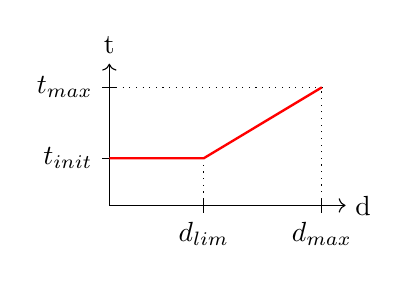
\begin{tikzpicture}[scale=3]
	\axes{d}{t}{1}{0.6}
	\valx{0.9}{$d_{max}$}
	\valx{0.4}{$d_{lim}$}
	\valy{0.2}{$t_{init}$}
	\valy{0.5}{$t_{max}$}
	\draw[dotted] (0.4,0.2) -- (0.4,0);
	\draw[line width = 0.3mm, color=red] (0,0.2)--(0.4,0.2) -- (0.9,0.5);
	\draw[dotted] (0,0.5) -- (0.9,0.5);
	\draw[dotted] (0.9,0) -- (0.9,0.5);
\end{tikzpicture}

%%%%%
\newpage

\newpage
\subsection{Expression du temps de parcours moyen}
Du noeud A au noeud B il y a n chemins, $c_1,...,c_n$\\
Le flux total, de 1, est répartit en flux sur chaque chemin ($d_1,d_2,...,d_n$
avec $\sum_{i=1}^n d_i=1$)\\
Les arètes du graphe sont des portions de route ($r_1,...,r_m$)\\
Les arètes disposent d'une fonction de temps de parcours en fonction du débit
entrant ($f_1,f_2,...,f_m$)\\
Les arètes disposent aussi d'un débit passant ($D_1,...,D_m$ tels que
$D_k = \sum_{i / r_k\in c_i} d_i$)\\
Alors le temps de parcours moyen du graphe est la moyenne pondérée du temps de
parcours de chaque chemin par le débit du chemin.\\
Le temps de parcours du chemin i est $t_i$ ($t_1,t_2,...,t_n$)\\
On peut exprimer $T_{tot}=\sum_{i=0}^n = d_i t_i$ et
$t_i = \sum_{k/r_k\in c_i} f_k(D_k)$ \\
Intoduisons $\xi_{i,k} = 1$ si l'arrête k appartient au chemin i et 0 sinon.\\
Alors, $D_k = \sum_{i=0}^n \xi_{i,k} d_i$ et
$t_i = \sum_{k=0}^m \xi_{i,k} f_k(D_k)$\\
On a finalement l'expression de la fonction $T_{tot}$ qui a n-1 variables
$d_1,...,d_{n-1}$ ($d_n = 1-\sum_{i=0}^n d_i$)
dont on tentera d'approcher le minimum.\\
$T_{tot}=\sum_{i=0}^n d_i \sum_{k=0}^m \xi_{i,k} f_k(\sum_{i=0}^n \xi_{i,k} d_i)$\\


\subsection{résolution par descente de gradient}
Pour ce qui est de la résolution pour des fonctions de ralentissement compliquées,
on se rammène àa minimiser la fonction qui à une repartition du débit sur les
différents chemins associe le temps de parcours moyen.\\
Considérons les chemins $c_1,\cdots,c_n$ dans un certain ordre et considérons
en entrée de notre fonction de temps de parcours moyen la répartition du débit
$d_1,d_2,\cdots,d_{n-1} \in [0,1]$, avec $\sum_{i=1}^n d_i = 1$. Si $d_i=0.2$
on dirige 20\% des voitures sur le chemin i.\\
Tout notre problème se rammène alors à trouver le minimum d'une fonction à
$n-1$ variables.\\
Nous pouvons espérer que notre fonction est différentiable en tout point de
$[0,1]^{n-1}$, pour ainsi avoir la possibilité d'utiliser l'algorithme de
descente de gradient, nous permettant de trouver à partir d'un point,
un minimum local. Alors une résolution approchée pourrait consister à
appliquer la descente de gradient à une multitude de points aléatoires et de
comparer les minimums locaux trouvés. Le résultat ne sera alors pas forcément
le minimum de la fonction mais on peut espérer qu'il s'en rapproche avec un
nombre conséquent de points.
\newpage

\subsection{graphes série/parallèle}
Un graphe série-parallèle est construit récursivement,
de la manière suivante :\\
C'est soit\\
-une simple route
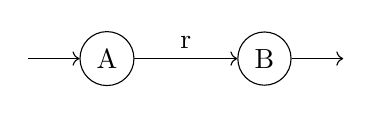
\begin{tikzpicture}[baseline=(current bounding box.center)]
    \node[shape=circle,draw=black] (A) at (0,0) {A};
    \node[shape=circle,draw=black] (B) at (2,0) {B};
    \draw [->] (-1,0) -- (A);
    \draw [->] (A) -- node[above]{r} (B);
    \draw [->] (B) -- (3,0);
\end{tikzpicture}\\
-deux sous graphes en parallèle
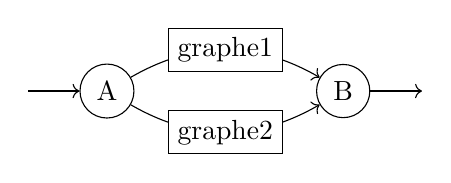
\begin{tikzpicture}[baseline=(current bounding box.center)]
    \node[shape=circle,draw=black] (A) at (0,0) {A};
    \node[shape=circle,draw=black] (B) at (3,0) {B};
    \draw [->] (-1,0) -- (A);
    \draw [->] (A) to[bend left] node[midway,draw,fill=white]{graphe1} (B);
    \draw [->] (A) to[bend right] node[midway,draw,fill=white]{graphe2} (B);
    \draw [->] (B) -- (4,0);
\end{tikzpicture}\\
-deux sous graphes en série
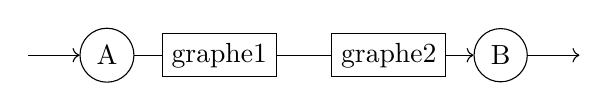
\begin{tikzpicture}[baseline=(current bounding box.center)]
    \node[shape=circle,draw=black] (A) at (0,0) {A};
    \node[shape=circle,draw=black] (B) at (5,0) {B};
    \draw [->] (-1,0) -- (A);
    \draw [->] (A) -- node[pos=0.25,draw,fill=white]{graphe1}
                        node[pos=0.75,draw,fill=white]{graphe2} (B);
    \draw [->] (B) -- (6,0);
\end{tikzpicture}\\
Pour tout aussi bien comprendre, voilà une implémentation en ocaml.
\begin{lstlisting}
    type graph_ser_paral =
         Route of arrete
        |Parallel of (graph_ser_paral*graph_ser_paral)
        |Serie of (graph_ser_paral*graph_ser_paral);;
\end{lstlisting}
Pour résoudre notre problème sur ce genre de graphe, on peut se rammener à 
résoudre les sous problèmes des sous graphes :\\
Pour le cas d'une simple route et le cas d'un graphe en série, on ne peut rien 
changer à la répartition des débit de voitures.\\
Pour le cas d'un graphe parallèle, on a un débit entrant (1 pour le graphe 
total) et on souhaite répartir ce débit sur les branches du graphe, on veut donc
déterminer $d_1$ et $d_2$ (avec $d_1+d_2=d$) pour que le parcours du graphe se
fasse en un temps minimal.\\
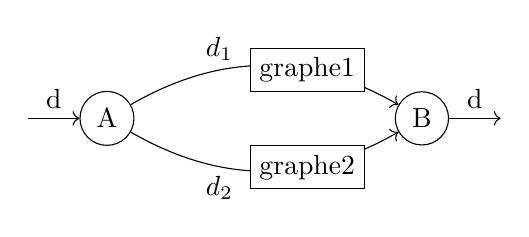
\begin{tikzpicture}[baseline=(current bounding box.center)]
    \node[shape=circle,draw=black] (A) at (0,0) {A};
    \node[shape=circle,draw=black] (B) at (4,0) {B};
    \draw [->] (-1,0) -- node[above]{d} (A);
    \draw [->] (A) to[bend left] node[pos=0.33,above]{$d_1$}
                    node[pos=0.66,draw,fill=white]{graphe1} (B);
    \draw [->] (A) to[bend right] node[pos=0.33,below]{$d_2$}
                    node[pos=0.66,draw,fill=white]{graphe2} (B);
    \draw [->] (B) -- node[above]{d} (5,0);
\end{tikzpicture}\\
Les fonctions de ralentissement du temps de parcours en fonction du débit peuvent
s'étendre par induction aux graphes parallèles, nous le verrons par la suite.
Soit $f_1$ celle du sous-graphe 1, $f_2$ celle du sous-graphe 2 et
$\widetilde{F}$ le temps de parcours du graphe parrallèle,
$\widetilde{F}(d,d_1) = \frac{d_1}{d}f_1(d_1)+\frac{d-d_1}{d}f_2(d-d_1)$ .\\A $d$ fixé, le but est de
trouver une valeur de $d_1$ pour que $\widetilde{F}(d,d_1)$ soit
minimum. Pour minimiser une fonction, on peut utiliser l'algorithme de
descente de gradient, pour lequel on a besoin de la dérivée :
$\frac{\partial \widetilde{F}}{\partial d_1}(d,d_1) = \frac{1}{d}(f_1(d_1) + d_1 f_1'(d_1) - f_2(d-d_1) + (d-d_1)f'_2(d-d_1)$
(qui suppose la dérivée de $f_1$ et celle de $f_2$ calculables).\\
On trouve alors $d_s$ cette valeur minimisant $\widetilde{F}$. $d_s$ dépend de
$d$. Alors, on obtient une fonction $F$ ne dépendant que de d.
$F(d)=f_1(d_s(d))+f_2(d-d_s(d))$
C'est cette fonction qui sera notre fonction de ralentissement du temps de parcours
du graphe série parallèle. $d_s(d)$ n'ayant à priori pas d'expression,
on ne pourra utiliser le calcul formel pour avoir la dérivée de $F$, on devra se
limiter à l'approximation de dérivées par $\frac{(x+h)-f(x)}{h}$ pour h assez
petit.

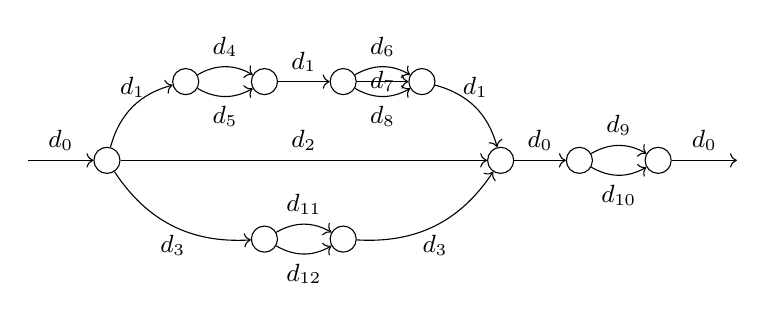
\begin{tikzpicture}[baseline=(current bounding box.center), font=\small]
	\node[shape=circle,draw=black,fill=white] (A) at (0,0) {};
	\node[shape=circle,draw=black,fill=white] (B) at (1,1) {};
	\node[shape=circle,draw=black,fill=white] (C) at (2,1) {};
	\node[shape=circle,draw=black,fill=white] (D) at (3,1) {};
	\node[shape=circle,draw=black,fill=white] (E) at (4,1) {};
	\node[shape=circle,draw=black,fill=white] (F) at (2,-1) {};
	\node[shape=circle,draw=black,fill=white] (G) at (3,-1) {};
	\node[shape=circle,draw=black,fill=white] (H) at (5,0) {};
	\node[shape=circle,draw=black,fill=white] (I) at (6,0) {};
	\node[shape=circle,draw=black,fill=white] (J) at (7,0) {};
	\draw [->] (A) to[bend left] node[above] {$d_1$} (B);
	\draw [->] (B) to[bend left] node[above] {$d_4$} (C);
	\draw [->] (B) to[bend right] node[below] {$d_5$} (C);
	\draw [->] (C) to node[above] {$d_1$} (D);
	\draw [->] (D) to[bend left] node[above] {$d_6$} (E);
	\draw [->] (D) to node {$d_7$} (E);
	\draw [->] (D) to[bend right] node[below] {$d_8$} (E);
	\draw [->] (E) to[bend left] node[above] {$d_1$} (H);
	\draw [->] (A) to node[above] {$d_2$} (H);
	\draw [->] (A) to[bend right] node[below] {$d_3$} (F);
	\draw [->] (F) to[bend left] node[above] {$d_{11}$} (G);
	\draw [->] (F) to[bend right] node[below] {$d_{12}$} (G);
	\draw [->] (G) to [bend right] node[below] {$d_3$} (H);
	\draw [->] (H) to node[above] {$d_0$} (I);
	\draw [->] (I) to[bend left]node[above] {$d_9$} (J);
	\draw [->] (I) to[bend right]node[below] {$d_{10}$} (J);
	\draw [->] (-1,0) to node[above] {$d_0$} (A);
	\draw [->] (J) to node[above] {$d_0$} (8,0);
\end{tikzpicture}\\


\end{document}
%http://www.msc.univ-paris-diderot.fr/~daerr/teaching/phynumM1/notes2cours/methodes_numeriques_MINI.pdf%